\documentclass[reprint]{revtex4-2}
\usepackage{braket,amsmath,amssymb,color,graphicx,bookmark,bm}
\begin{document}

\title{Iterative Ground State Approach Algorithm}
\author{Abhirup Mukherjee}
\affiliation{EPQM}
\begin{abstract}
	The following is the algorithm for performing an iterative diagonalization of fermionic systems. It is mostly similar to DMRG and NRG, and allows obtaining the low-energy spectrum of large many-body Hamiltonians.
\end{abstract}
\date{\today}
\maketitle

\section{Introduction}
The broad idea is the following. We have a Hamiltonian describing an interacting set of states (in real or momentum space). We can express the total Hamiltonian in an incremental fashion: \(H = \sum_i H_i\), where \(H_{i+1}\) involves more number of states than \(H_i\). For example, a tight-binding model can be written in that form, with the definition \(H_i = c^\dagger_{i+1}c_i + \text{h.c.}\). The iterative diagonalisation method obtains the low-energy spectrum of this problem in the following manner: We first diagonalise the Hamiltonian \(H\) for a smaller value of \(i\), small enough such that this can be done exactly. We then truncate the spectrum to a predefined size, and rotate all existing operators to this truncated basis, including the Hamiltonian \(H\). We then consider the "bonding Hamiltonian" \(\Delta H\) between the existing sites and the new sites, and rotate the same into the truncated basis. Adding the previous rotated Hamiltonian \(H\) and the rotated increment Hamiltonian \(\Delta H\) gives us a truncated but effective Hamiltonian for the increased number of sites. We again diagonalise this, and again retain only a fixed number of states in the spectrum. We keep repeating this until we reach the required number of sites.


\section{Structure of Hamiltonian and Operators}
\subsection{Jordan-Wigner Matrix Representation of Fermionic Operators}
For a single qubit, the creation/annihilation matrices are
\begin{equation}\begin{aligned}
	c = \begin{pmatrix}0 & 1 \\ 0 & 0\end{pmatrix}, c^\dagger = \begin{pmatrix}0 & 0 \\ 1 & 0\end{pmatrix}~,
\end{aligned}\end{equation}
given the convention that \(\ket{1} = (0 ~ ~ 1)\) is the occupied state. For a many-body system, these must be replaced with field operators that have the canonical fermionic algebra. For a system of \(N\) 1-particle levels, this can be accomplished through a {\it Jordan-Wigner}-like transformation
\begin{equation}\begin{aligned}
	c_j = \left(\otimes_1^j \sigma_z\right) \otimes c \otimes \left(\otimes_1^{N-j} \mathbb{I}\right) ~, j \in [0, N-1]~,
\end{aligned}\end{equation}
where \(\sigma_z = \begin{pmatrix} 1 & 0 \\ 0 & -1 \end{pmatrix} \) and \(\mathbb{I} = \begin{pmatrix} 1 & 0 \\ 0 & 1 \end{pmatrix} \). For example, for spinless electrons on a three-site lattice, we can have three fermionic operators: \(c_{1}\),\(c_{2}\), and \(c_{3}\). Following the above expression, their matrices are\\
\begin{equation*}\begin{aligned}
	c_1 = c \otimes \mathbb{I} \otimes \mathbb{I} = \begin{bmatrix}
0 & 0 & 1 & 0 & 0 & 0 &  0 &  0 \\
0 & 0 & 0 & 1 & 0 & 0 &  0 &  0 \\
0 & 0 & 0 & 0 & 0 & 0 &  0 &  0 \\
0 & 0 & 0 & 0 & 0 & 0 &  0 &  0 \\
0 & 0 & 0 & 0 & 0 & 0 & -1 &  0 \\
0 & 0 & 0 & 0 & 0 & 0 &  0 & -1 \\
0 & 0 & 0 & 0 & 0 & 0 &  0 &  0 \\
0 & 0 & 0 & 0 & 0 & 0 &  0 &  0 
\end{bmatrix}~,\\
	c_2 = \sigma \otimes c \otimes \mathbb{I} = \begin{bmatrix}
0 & 0 & 1 & 0 & 0 & 0 &  0 &  0 \\
 0 & 0 & 0 & 1 & 0 & 0 &  0 &  0 \\
 0 & 0 & 0 & 0 & 0 & 0 &  0 &  0 \\
 0 & 0 & 0 & 0 & 0 & 0 &  0 &  0 \\
 0 & 0 & 0 & 0 & 0 & 0 & -1 &  0 \\
 0 & 0 & 0 & 0 & 0 & 0 &  0 & -1 \\
 0 & 0 & 0 & 0 & 0 & 0 &  0 &  0 \\
 0 & 0 & 0 & 0 & 0 & 0 &  0 &  0 
\end{bmatrix}~,\\
		c_3 = \sigma \otimes \sigma \otimes c = \begin{bmatrix}
	0 & 1 & 0 &  0 & 0 &  0 & 0 & 0 \\
	0 & 0 & 0 &  0 & 0 &  0 & 0 & 0 \\
	0 & 0 & 0 & -1 & 0 &  0 & 0 & 0 \\
	0 & 0 & 0 &  0 & 0 &  0 & 0 & 0 \\
	0 & 0 & 0 &  0 & 0 & -1 & 0 & 0 \\
	0 & 0 & 0 &  0 & 0 &  0 & 0 & 0 \\
	0 & 0 & 0 &  0 & 0 &  0 & 0 & 1 \\
	0 & 0 & 0 &  0 & 0 &  0 & 0 & 0 
\end{bmatrix}~,\\
\end{aligned}\end{equation*}

For later use, we define the {\it antisymmetriser matrix} \(S(j)\) and identity matrix \(\mathbb{I}(j)\),
\begin{equation}\begin{aligned}
	S(j) &= \otimes_1^j \sigma_z = \sigma_z \otimes \ldots j\text{ times } \ldots \otimes \sigma_z,\\
	\mathbb{I}(j) &= \otimes_1^{N-j} \mathbb{I} = \mathbb{I} \otimes  \ldots j\text{ times } \ldots \otimes \mathbb{I}~,
\end{aligned}\end{equation}
to express the fermionic representation compactly:
\begin{equation}\begin{aligned}\label{jordanwigner}
	c_j = S(j) \otimes c \otimes \mathbb{I}(N-j)~.
\end{aligned}\end{equation}

\subsection{Structure of Hamiltonian}
We consider a general impurity model, of \(L\) number of sites (excluding the impurity site):
\begin{equation}\begin{aligned}\label{hamiltonian}
	H_\text{sys}(L) = H_\text{imp} + H_\text{imp-bath} +  
	- t\sum_{\sigma, j = 1}^{L-1}\left(c^\dagger_{j,\sigma}c_{j+1,\sigma} + \text{h.c.}\right) ~,
\end{aligned}\end{equation}
where \(H_\text{imp}\) is the Hamiltonian for the decoupled impurity site and \(H_\text{imp-bath}\) is the impurity-bath coupling. Such a system has \(2L+2\) single-particle levels in the full system (2 spin levels for each of the \(L+1\) sites).

Iteration scheme (the initial number of states is \(L_0\)):
\begin{equation}\begin{aligned}\label{iterationScheme}
	H_0(L_0) &= H_\text{sys}(L_0)~,\\
	H_{r+1}(L_0) &= H_r(L_0) + \Delta H_r(L_0), ~ r \geq 0~,\\
	\Delta H_r(L_0) &= - t\sum_{\sigma}\left(c^\dagger_{L_0 + r,\sigma}c_{L_0 + r+1,\sigma} + \text{h.c.}\right).
\end{aligned}\end{equation}
\(H_0\) is the initial Hamiltonian, consisting of \(L_0\) lattice sites in the bath, \(H_{r+1}(L_0)\) is the Hamiltonian after \(r+1\) iterations having started with \(L_0\) sites, and \(\Delta H_r(L_0)\) is the increment term that gets added to \(H_r(L_0)\) during the \((r+1)^\text{th}\) iteration to give rise to \(H_{r+1}(L_0)\). 

%\section{Getting Together Everything That We Need}
%The broad idea of the algorithm (described in the next section) is the following: At any given step, we diagonalise the Hamiltonian for a given number of step, truncate the set of eigenstates to a manageable size, transform all operators to this rotated truncated basis, add a new site to the model to generate a new Hamiltonian, and then start from the first step. In preparation for describing the algorithm in more detail, we now describe various mathematical objects that we will use in the process.
%
%\subsection{Specifications}
%\begin{itemize}
%	\item \(H_r\) is the Hamiltonian at the start of any given step \(r\) of the iteration.
%	\item \(D_\text{tr}\) is the maximum number of eigenstates that are retained from any single symmetry sector any given step of the iteration.
%	\item The basis for representing the Hamiltonian at any given step is denoted as \(\mathcal{B}_r\). Its dimensions are \(D_r \times N_r\), obtained by stacking the basis vectors column-wise:
%\begin{equation}\begin{aligned}
%	\mathcal{B}_r = \left[\underbrace{V_1}_{D_r \times 1};\quad V_2; \quad \ldots V_{N_r}\right]_{D_r \times N_r} ~,
%\end{aligned}\end{equation}
%where \(V_1, V_2\), etc are the basis vectors represented as column vectors.
%	\item We start the iteration by considering \(L_0\) sites in the conduction bath, the initial Hamiltonian being \(H_0(L_0)\).
%\end{itemize}
%
%\subsection{Using Symmetries}
%Typically, our Hamiltonians will enjoy a global \(U(1)\) symmetry (overall number conservation) and overall magnetisation conservation. This will be preserved under the transformations, and will hold for the Hamiltonian at any step. We can therefore classify our basis \(\mathcal{B}_r\) into sectors \(\left\{\mathcal{B}_r^{(\nu)}\right\} \) according to the quantum numbers \(\nu\) of the symmetries. For the above example of total particle number conservation and total magnetisation conservation, \(\nu\) refers to the tuples \((N, m_z)\) of eigenvalues of the total number operator and the total magnetisation operator. The size (dimension) of each basis vector is \(D_r\).
%
%We are also gonna need to track the indices \(C^{(\nu)}\) of the columns of \(\mathcal{B}_r\) at which a particular subspace \(\mathcal{B}_r^{(\nu)}\) has non-zero values. As an illustration, consider the following artificial example where the values \(x_i\) form the symmetry block with \(\nu=1\), \(z\) forms the block \(\nu=2\) and \(y_i\) form \(\nu=3\):
%\begin{equation}\begin{aligned}
%	\mathcal{B}_r = \begin{bmatrix} 
%		x_1 & x_3 & 0 & 0 & 0 \\
%		x_2 & x_4 & 0 & 0 & 0 \\
%		0 & 0 & z & 0 & 0 \\
%		0 & 0 & 0 & y_1 & y_1 \\
%		0 & 0 & 0 & y_2 & y_2 \\
%	\end{bmatrix} ~,\quad
%	\mathcal{B}_r^{(1)} = \begin{bmatrix} 
%		x_1 & x_3 \\
%		x_2 & x_4 \\
%		0 & 0 \\
%		0 & 0 \\
%		0 & 0 \\
%	\end{bmatrix} ~,\quad
%	\mathcal{B}_r^{(2)} = \begin{bmatrix} 
%		0 \\
%		0 \\
%		z \\
%		0 \\
%		0 \\
%	\end{bmatrix} ~,\quad
%	\mathcal{B}_r^{(3)} = \begin{bmatrix} 
%		0 & 0 \\
%		0 & 0 \\
%		0 & 0\\
%		y_1 & y_1 \\
%		y_2 & y_2 \\
%	\end{bmatrix} ~,\quad
%	\begin{aligned}
%	& C^{(1)} =[1, 2],\\
%	& C^{(2)} =[3], \\
%	& C^{(3)} =[4, 5]~.
%    \end{aligned}
%\end{aligned}\end{equation}
%
%\subsection{Adding new sites}
%We also have \(L_r + 1\) fermionic field operators \(\left\{ c_j \right\} \), written in the basis \(\mathcal{B}_r\) at any given step, where \(L_r\) is the number of lattice sites present in the system at this step. These operators act on \(L_r+1\) number of sites; in order to go from one step of the iteration to the next, we will need to expand the system by adding one or more sites. This addition of sites requires the antisymmetrization of new field operators (acting purely on the new sites) against the existing \(L_r + 1\) operators (acting on the old sites). This antisymmetrization, in turn, requires a large antisymmetrization operator \(S_r = \otimes_1^{L_r+1}\sigma_z\).

\section{The Algorithm}
\subsection{Iterative Diagonalization}
Let the starting Hamiltonian be \(H_0(L_0)\), consisting of \(L_0\) single-particle levels (hence a Hilbert space dimension of \(2^{L_0}\)). We start with a single-particle computational basis and construct the \(L_0\) fermionic operators \(c_1, c_2, \ldots, c_{L_0}\) in this basis, using eq.~\ref{jordanwigner}. We also keep track of a large antisymmetriser matrix \(S(L_0)\) that will be used to attach new sites when we expand the system. Let \(M_s\) be the maximum number of eigenstates we retain in the spectrum at any given step. The value of \(M_s\) should be chosen so that a \(M_s\times M_s\) matrix can be diagonalised in reasonable time.
\begin{itemize}
	\item[{\it S1.}] Construct the complete Hamiltonian matrix \(H_0\) in our present basis using the field operators \(\left\{c_j\right\}\). Diagonalise the Hamiltonian (of size \(D_0 \times D_0\)) and obtain the eigenvalues \({E_n}\) and eigenstates \({X_n}\). Each \(X_n\) is a column vector of size \(D_0\).
	\item[{\it S2.}] Retain at most \(M_s\) number of eigenstates, preferring the ones with lower energy. The reduced basis for this rotated truncated subspace is constructed by stacking the column vectors \(X_n\) horizontally:
		\begin{equation}\begin{aligned}\label{rotationMatrix}
			R = [X_1 X_2 \ldots X_{M_s}]_{D_0\times M_s}~.
		\end{aligned}\end{equation}
		This matrix also acts as the transformation to rotates and truncate all operators from the old basis into the new one.
	\item[{\it S3.}] We rotate our Hamiltonian \(H_0\), our fermionic operators \(\left\{ c_j \right\} \) and the large antisymmetrizer matrix \(S(L_0)\) into the new reduced basis, using the transformation \(\mathcal{O} \to R^\dagger \mathcal{O} R\).
	\item[{\it S4.}] We now need to expand our system by adding the increment Hamiltonian \(\Delta H_0\). Let the number of {\it new } 1-particle levels in \(\Delta H_0\) be \(L_\Delta\). These new levels will be indexed as \(L_0+1,\ldots,L_0+L_\Delta\). We need to define antisymmetrized fermionic operators for the new sites:
		\begin{equation}\begin{aligned}
			c_{L_0+1} &= c \otimes \mathbb{I}(2^{L_\Delta - 1}),\\
			c_{L_0+2} &= \sigma_z \otimes c \otimes \mathbb{I}(2^{L_\Delta - 2}),\\
					   &~~ \ldots~\\
			~c_{L_0+L_\Delta} &= (\otimes_1^{L_\Delta-1} \sigma) \otimes c ~.
		\end{aligned}\end{equation}
		These have to be calculated in the local computational basis (of size \(2^{L_\Delta}\)) of the new levels. 
	\item[{\it S5.}] Combining the new sites with the old sites leads to a combined Hilbert space dimension of \((M_s + 2^{L_\Delta}) \times (M_s + 2^{L_\Delta})\). To allow all operators to act on the enlarged Hilbert space, we expand both sets of operators:
	\begin{equation}\begin{aligned}
		c_j &= S(L_0) \otimes c_j;~~j=L_0 +1, \ldots, L_\Delta~,\\
		c_j &= c_j \otimes \mathbb{I}(2^{L_\Delta});~ ~ j=1, 2, \ldots, L_0~,\\
		H_0 &\to H_0 \otimes \mathbb{I}(2^{L_\Delta}),\\
		S(L_1) &= S(L_0) \otimes \mathbb{I}(2^{L_\Delta})~.
	\end{aligned}\end{equation}
	where \(\mathbb{I}(2^{L_\Delta})\) is an identity matrix of dimension \(2^{L_\Delta} \times 2^{L_\Delta}\). Note that the operators in the last three equations are the rotated ones (following Step 3).
\item[{\it S6.}] Using the transformed operators \(c_{L_0+1},\ldots,c_{L_0 + L_\Delta}\) for the new sites, construct the difference Hamiltonian matrix \(\Delta H_0\) and hence the updated Hamiltonian \(H_1 = H_0 + \Delta H_0\) for the next step. Repeat the process starting from step 2 with the new Hamiltonian \(H_1\), the new operators \(c_j\) and the new matrix \(S(L_1)\) replacing the old counterparts.
\end{itemize}

\subsection{Static Correlations}
We are in general interested in \(n-\)point correlations of the form \(\left<\mathcal{O}_1 \mathcal{O}_2 \ldots \mathcal{O}_n\right>\), where \(\mathcal{O}_i\) are operators that act on 1-particle Hilbert spaces. Let the earliest step of the iterative diagonalisation procedure at which all these operators have entered the system be \(r\). At this step \(r\), construct the correlation operator \(\mathcal{O}_1 \mathcal{O}_2 \ldots \mathcal{O}_n\) using the fermionic matrices \(c_j\) at that step (recall that these matrices will be highly rotated versions of the matrices we started with). Having constructed the operator \(O\), we expand and rotate it after the completion of every future step: \(O_{n+1} = (R_n^\dagger O_n R_n)\otimes \mathbb{I}(2^{L_\Delta})\), where \(R_n\) is the rotation matrix for the \(n^\text{th}\) step. The last step \(n^*\) of the iterative diagonalisation consists of only a diagonalisation and no expansion, resulting in a final set of eigenstates \(\left\{ X_i \right\} \). The form of the correlation operator in this basis is \(O_{n^*} = R^\dagger_{n^*-1} O_{n^*-1} R_{n^*}\). The expectation value can now be calculated using the matrix \(O_{n^*}\) and the ground state of \(\left\{ X_i \right\} \).

\section{Examples and Benchmarks}
\subsection{Single-Impurity Anderson Model}
The single-impurity Anderson model at half-filling is obtained by setting \(H_\text{imp}=-\frac{U}{2}\left(n_{d \uparrow} - n_{d \downarrow}\right)^2 \) and \(H_\text{imp-bath} = -V\sum_\sigma \left(c^\dagger_{d\sigma}c_{0\sigma} + \text{h.c.}\right)\) in eq.~\ref{hamiltonian}. We studied this model using the above approach to benchmark the ground state energy and spin-flip correlation \(\left<\frac{1}{2}S_d^+ S_0^- + \text{h.c.} \right>\) against exact diagonalization (ED). In order to extend the ED to a larger number of sites, we restricted ourselves to just the \(N=2\) sector, \(N\) being the total occupancy. We find very good agreement for \(M_s \sim 1000\) and above. These results are shown in Fig.~\ref{comparisonSIAM}.
\begin{widetext}
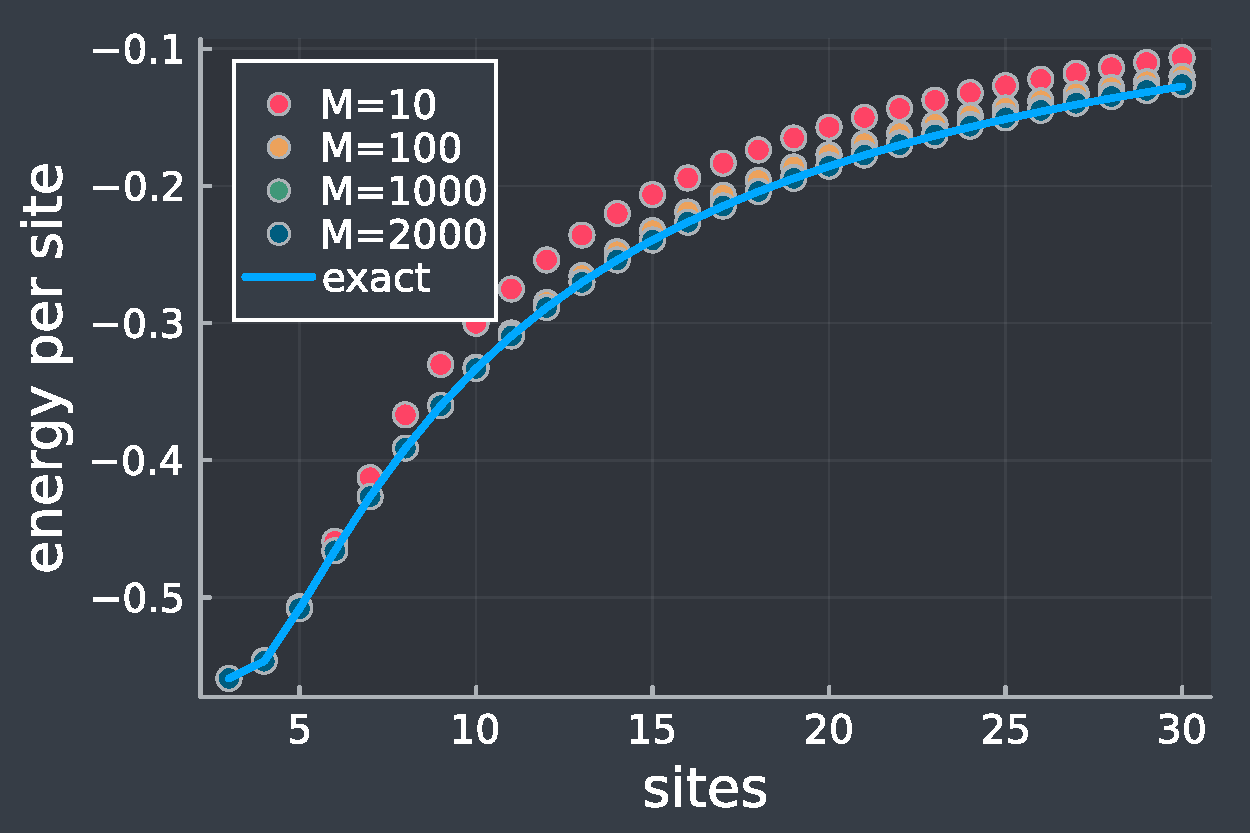
\includegraphics[width=0.48\textwidth]{energy.pdf}
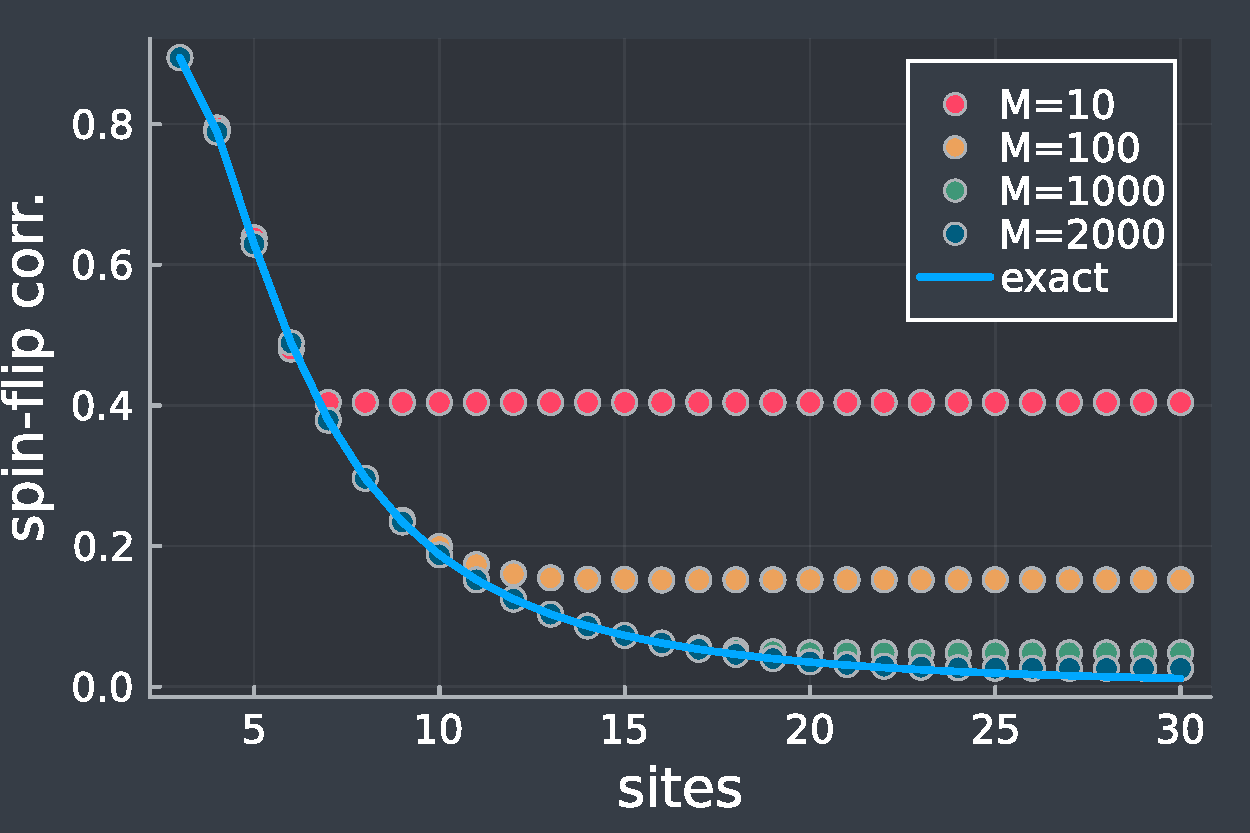
\includegraphics[width=0.48\textwidth]{spinflipcomparison.pdf}
\label{comparisonSIAM}
\end{widetext}

\section{Transforming Across Reduced Bases}
\subsection{The problem of mixing states across Hamiltonians}
Consider the following problem: We have a quantum impurity problem that undergoes a transition from a Kondo-screened phase to a local moment phase through a critical point, and we wish to study the nature of the critical point. In order to take account of the enhanced fluctuations arising at the critical point because of the degeneracy between the Kondo-screened ground state \(\ket{\Psi_\text{KS}}\) and the local moment state \(\ket{\Psi_\text{LM}}\), it is helpful to use a superposition ground state, of the form
\begin{equation}\begin{aligned}\label{superposition}
	\ket{\Psi_c} = \frac{1}{\sqrt 2}\left(\ket{\Psi_\text{KS}} + \ket{\Psi_\text{LM}}\right) ~.
\end{aligned}\end{equation}
More explicitly, \(\ket{\Psi_\text{KS}}\) and \(\ket{\Psi_\text{LM}}\) are obtained as ground states of the low-energy Hamiltonians \(H_\text{KS}\) and \(H_\text{LM}\) in the Kondo-screened and local moment phases respectively. If we use the iterative diagonalisation algorithm described above to obtain these states, the state vectors will be represented in terms of inconsistent basis states. That is, \(\ket{\Psi_\text{KS}}\) will be represented in terms of the eigenstates of \(H_\text{KS}\), while \(\ket{\Psi_\text{LM}}\) will be available in terms of the eigenstates of \(H_\text{LM}\), making the addition operation in eq.~\ref{superposition} tricky (we can only add two column vectors if they are in the same basis).

\subsection{Basis transformation of states}
In order to remedy this, it is necessary to transform one of the states into the basis of the other. Suppose we are given two states \(\ket{\Psi^{(1)}}\) and \(\ket{\Psi^{(2)}}\) written in two basis sets \(\left\{ \ket{b^{(1)}_i}\right\} \) and \(\left\{ \ket{b^{(2)}_i}\right\} \),
\begin{equation}\begin{aligned}
	\ket{\Psi^{(1)}} = \begin{pmatrix} c_1^{(1)} ~ c_2^{(1)} ~ \ldots ~ c_N^{(1)} \end{pmatrix}^T = \sum_i c_i^{(1)} \ket{b_i^{(1)}},\\
	\ket{\Psi^{(2)}} = \begin{pmatrix} c_1^{(2)} ~ c_2^{(2)} ~ \ldots ~ c_N^{(2)} \end{pmatrix}^T = \sum_i c_i^{(2)} \ket{b_i^{(2)}}.
\end{aligned}\end{equation}
We can transform \(\ket{\Psi^{(1)}}\) into the basis \(\left\{ \ket{b^{(2)}_i}\right\} \) by inserting an identity resolution:
\begin{equation}\begin{aligned}
	\ket{\Psi^{(1)}} &= \sum_{i, j} c_i^{(1)} \ket{b_j^{(2)}}\braket{b_j^{(2)}|b_i^{(1)}} \\
					 &= \sum_{j} \left(\sum_i c_i^{(1)} M^{2, 1}_{ji} \right)\ket{b_j^{(2)}},
\end{aligned}\end{equation}
where \(M^{2, 1}_{ji} = \braket{b_j^{(2)}|b_i^{(1)}}\). This can also be represented as a matrix multiplication operation:
\begin{equation}\begin{aligned}\label{stateTransform}
	\Psi^{(1)}\vert_{1} \to \Psi^{(1)}\vert_{2} = \hat M^{2, 1}~\Psi^{(1)}\vert_{1}~,
\end{aligned}\end{equation}
where \(\Psi^{(1)}\vert_{1}\) and \(\Psi^{(1)}\vert_{2}\) are the column vector representations of the state \(\ket{\Psi^{(1)}}\) in the first basis and second basis respectively, and \(\hat M^{2, 1}\) is the matrix (obviously in the first basis, since it is multiplied with a state in that basis) defined by the matrix elements \(\hat M^{2, 1}_{ij} = \braket{b_i^{(2)} | b_j^{(1)}}\). In summary, eq.\ref{stateTransform} is the recipe for transforming the representation of a state from one basis to another.
	
\subsection{The problem of incompatible basis sets}
Formulating eq.~\ref{stateTransform} above for the problem laid out in the first part of this section, we interpret \(\ket{\Psi_\text{LM}}\) as \(\ket{\Psi^{(1)}}\) (the state whose representation needs to be modified), and we interpret the two basis sets \(\left\{ \ket{b^{(1)}_i}\right\}\) and \(\left\{ \ket{b^{(2)}_i}\right\}\) as the eigenbasis of \(H_\text{LM}\) and \(H_\text{KS}\) respectively:
\begin{equation}\begin{aligned}
	\left\{ \ket{b^{(1)}_i}\right\} &= \left\{ \ket{b^{\text{LM}}_i}\right\}\\
	\left\{ \ket{b^{(2)}_i}\right\} &= \left\{ \ket{b^{\text{KS}}_i}\right\}~.
\end{aligned}\end{equation}
More specifically, the iterative diagonalisation of \(H_\text{LM}\) will lead to a sequence of Hamiltonians (with increasing number of one-particle states), and the eigenbasis of each such Hamiltonian acts as the basis for the next Hamiltonian in the sequence (the initial Hamiltonian is written in the local computational basis); \(\left\{ \ket{b^{\text{LM}}_i}\right\}\) is then the basis in which the final Hamiltonian and its ground state is expressed (before it is diagonalised). Same holds for the other Hamiltonian \(H_\text{KS}\) and the basis \(\left\{ \ket{b^{\text{KS}}_i}\right\}\).

The creation of the matrix \(\hat M\) requires the calculation of inner products between basis vectors of two distinct basis sets. This can be carried out in practise only if the vectors of both sets are themselves represented in a common basis (the inner product is essentially the multiplication of a row matrix with a column matrix, and the two matrices must be written in the same basis). This reveals a problem in the application of eq.~\ref{stateTransform} directly to the problem at hand: a calculation of the kind 
\begin{equation}\begin{aligned}
	\hat M^{\text{KS}, \text{LM}}_{i,j} = \braket{b^{\text{KS}}_i | b^{\text{LM}}_j}~,
\end{aligned}\end{equation}
followed by
\begin{equation}\begin{aligned}
	 \ket{\Psi_\text{LM}} \to \hat M^{\text{KS},\text{LM}}\ket{\Psi_\text{LM}}~,
\end{aligned}\end{equation}
is incorrect; this is because, the final basis sets in the iterative diagonalisation of the two Hamiltonians are written in the next to last basis set of the same Hamiltonian, which means that \(\left\{ \ket{b^{\text{LM}}_j}\right\}\) and \(\left\{ \ket{b^{\text{KS}}_i}\right\}\) are not available in the same basis.

\subsection{Transforming both states to a common basis}
As pointed out above, it is not possible to directly construct a basis transformation operator \(\hat M\) that places both \(\ket{\Psi_\text{LM}}\) and \(\ket{\Psi_\text{KS}}\)  in the same basis. We therefore adopt a different strategy: we will transform both the states, individually, to the completely local single-particle basis (CLSB). This CLSB is, in fact, the starting point of any iterative diagonalisation procedure - it is the basis in which the first Hamiltonian of the flow is constructed. 

For concreteness, let the basis set in which the \(j^\text{th}\) Hamiltonian \(H_j\) is written be \(B_j\). An important point is that the explicit basis vectors of the set \(B_j\) are available (during the actual computation) only in the earlier basis (even though \(H_j\) itself is written using the \(j^\text{th}\) basis). This continues all the way back to \(B_2\), where \(B_2\) is the second basis set and is represented in terms of the CLSB \(B_1\); \(B_1\) is written in its own basis.

Let the final ground state (after the \(N^\text{th}\) diagonalisation) be \(\ket{\Psi_N^{(N)}}\). The superscript indicates that the state is computationally expressed in the basis \(B_N\). The first step is to express this state in the basis \(B_{N-1}\). Following our earlier discussion, this can be achieved through
\begin{equation}\begin{aligned}
	\ket{\Psi_N^{(N)}} \to \ket{\Psi_N^{(N - 1)}} = \hat M^{N-1, N}\ket{\Psi_N^{(N)}}~,
\end{aligned}\end{equation}
where the basis transformation matrix is expressed in the basis \(B_N\), and its elements are given by
\begin{equation}\begin{aligned}\label{actualTransform}
	\hat M^{N-1, N}_{i, j} = \braket{B_{N-1, i}^{(N-1)} | B_{N, j}^{(N-1)}}~;
\end{aligned}\end{equation}
the subscripts indicate that the state is the \(i^\text{th}\) (or the \(j^\text{th}\)) basis vector the \((N-1)^\text{th}\) (or the \(N^\text{th}\) basis set. The superscript indicates that both the basis vectors are computationally represented in the \((N-1)^\text{th}\) basis. This of course means that the basis vectors of \(B_{N-1}\) will be very simple. Assuming there as \(D\) states in \(B_{N-1}\), we have
\begin{equation}\begin{aligned}\label{identity}
	B_{N-1} = \left\{ \begin{pmatrix} 1 \\ 0 \\ \vdots \\ 0\end{pmatrix}, \begin{pmatrix} 0 \\ 1 \\ \vdots \\ 0\end{pmatrix} \ldots \begin{pmatrix} 0 \\ 0 \\ \vdots \\ 1\end{pmatrix}\right\} = \left\{ P^1_D, P^2_D, \ldots, P^D_D \right\} ~,
\end{aligned}\end{equation}
where \(P^i_D\) is the vector of size \(D\) with 1 at the \(i^\text{th}\) position and zeros elsewhere. 

More specifically, let's say that we are retaining \(M_s\) number of eigenstates at each step of the iterative diagonalisation process. By diagonalisating the Hamiltonian \(H_{N-1}\) (which is written in the basis \(B_{N-1}\)), we obtain \(M_s\) eigenstates \( \left\{ \ket{e^i_{N-1}}; i=1,2,\ldots,M_s\right\} \). If we insert, say, another qubit into the system for the next step, we can only retain at most \(M_s/2\) of these eigenstates (the qubit itself will increase the number of states by a factor of 2, leading to the required \(M_s\) number of basis states). The complete basis \(B_{N}\) is obtained by rotating and truncating the existing system into the basis \(\left\{\ket{e^i_{N-1}}; i=1,2,\ldots,M_s/2\right\}\) and then taking the direct product of these states with the CLSB of the newly added qubit, which is just identity \(\mathbb{I}(2)\):
\begin{equation}\begin{aligned}\label{Nthstep}
	B_{N} = \left\{\ket{e^i_{N-1}}; i=1 \to M_s/2\right\}  \otimes \mathbb{I}(2)~.
\end{aligned}\end{equation}
The representation of \(B_N\) is therefore sort of hybrid - it uses the basis \(B_{N-1}\) for the old qubits (\(M_s/2\) states)	but uses the CLSB for the newly added qubit (2 states). That's just because the newly added qubit wasn't available when \(B_{N-1}\) was constructed, so the old basis \(B_{N-1}\) cannot account for that. In order to use eq.~\ref{actualTransform}, \(B_{N-1}\) and \(B_N\) must be in the same representation and of the same dimensions.  For the older qubits, we have \(B_{N-1} = \mathbb I(M_s/2)\) (via eq.~\ref{identity}). For the new qubits, we again use the CLSB, which leads to the full \(B_{N-1}\),
\begin{equation}\begin{aligned}\label{brokenidentity}
	B_{N-1} = \mathbb I(M_s/2) \otimes \mathbb I(2) = \left\{ P^i_{M_s}; i=1\to M_s \right\} ~,
\end{aligned}\end{equation}
which keeps eq.~\ref{identity} unchanged but gives us a clearer picture of what's going on. In fact, we can simplify eq.~\ref{actualTransform} by combining eqs.~\ref{Nthstep} and \ref{brokenidentity}. Since the new qubits are represented by identity matrices in both basis sets, it is only the old qubits whose states changes during the basis transformation. Therefore, the full transformation matrix \(\hat M^{N-1, N}\) can be split into two parts, one for the old qubits and one for the new qubits:
\begin{equation}\begin{aligned}
	\hat M^{N_1, N} \otimes \mathbb{I}(2),~\hat M^{N-1, N}_{i, j} = \braket{P^i_{M_s/2} | e^j_{N-1}}~.
\end{aligned}\end{equation}
The structure of the matrix element implies that the matrix \(\hat M^{N-1, N}\) has the eigenvectors \(\ket{e^j}\) as its columns. We conclude from this that the matrix \(\hat M^{N-1, N}\) is simply the diagonalising matrix \(R^{N-1}\) obtained after diagonalisation of the Hamiltonian \(H_{N-1}\) (see eq.~\ref{rotationMatrix}).

None of the arguments was specific to the final step of the iterative diagonalisation procedure, so we can immediately write down the general expressions for transforming a state \(\ket{\Psi_N^n}\) from \(B_n\) to \(B_{n-1}\):
\begin{equation}\begin{aligned}
\ket{\Psi_N^{(n)}} \to \ket{\Psi_N^{(n - 1)}} = \left( R^{n-1} \otimes \mathbb{I}(\Delta) \right) \ket{\Psi_N^{(n)}},
\end{aligned}\end{equation}
where \(\Delta\) is the number of states that must be padded in order to make up the correct dimension of the transformation operator.







\end{document}
